\documentclass[a4paper]{article}
\usepackage{graphicx} \usepackage{caption} \usepackage{pdfpages} \usepackage{pdflscape} \usepackage[margin=0.8in]{geometry} \usepackage{fancyhdr} \usepackage{pdfpages}
\usepackage{amsmath} \usepackage{lastpage}
\begin{document}
\pagestyle{fancy}
\fancyfoot[RO, LE] {\thepage\ of \pageref{LastPage}}
\fancyhead[LO,LE]{Design Specification, 1.1, Release} %Name of doc, version, draf/release
\fancyfoot[C]{Aberystwyth University / Computer Science} %Footer - no changes necessary
\begin{center}
\textsc{\LARGE The Software Development Life Cycle}\\[1.5cm]
\includegraphics[width=0.15\textwidth]{img/monster.png}\\[1.5cm] %Monster image
\textsc{\Large Monster Mash - Design Specification}\\[0.5cm] %Edit for document title

\begin{minipage}{0.8\textwidth}
\begin{flushleft} \large
\emph{Authors:}\\
James \textsc{Bowcott}\\
Marcus \textsc{Harrison}\\
Kamilia \textsc{Tacickaja}\\
%Repeat above line for more authors
\end{flushleft}
\end{minipage}
\vspace{8 mm}

\begin{minipage}{0.8\textwidth}
\begin{flushleft} \large
\emph{Task ID:}
SE\_03\_DESIGN\_DOCUMENT
\end{flushleft}
\end{minipage}
\vspace{8 mm}

\begin{minipage}{0.8\textwidth}
\begin{flushleft} \large
\emph{Version:}
1.1
\end{flushleft}
\end{minipage}
\vspace{8 mm}

\begin{minipage}{0.8\textwidth}
\begin{flushleft} \large
\emph{Status:}
Release
\end{flushleft}
\end{minipage}
\vspace{8 mm}

%Computer Science Dept Address
\begin{minipage}{0.8\textwidth}
\begin{flushleft} \large
Department of Computer Science\\
Aberystwyth University\\
Aberystwyth\\
Ceredigion\\
SY23 3DB\\
\end{flushleft}
\end{minipage}
\vfill
{\large \today}
\end{center}
\clearpage
\setlength\parindent{0pt}

\tableofcontents

%--------------------------------------------------------------------

\clearpage
\section{Introduction}

\subsection{Purpose of this Document}
The purpose of this document is to describe the design of the implementation for the Monster Mash group project, as described by the project requirements.\\

It should explain the system architecture, the significant modules of the system, and how they interact with each other to form a working implementation.

\subsection{Scope}
This document explains the chosen architectural design for the application, describes the significant modules that form as part of that design, and explains how they fulfil the functional requirements of the project specification.\\

The modules will be described to some level of detail, so that programmers have a basic understanding of those modules and how they fit into the system architecture and how they can program to them. It does not explicitly document every function or attribute of each module.\\

Diagrams will be included to show how these modules relate to and depend on each other.\\

Specific details of the implementation will be described in more detail, such as algorithms and the data model.


\subsection{Objectives}
To achieve the goals above, this document must meet the following objectives:
\begin{itemize}
\item Describe the architecture of the system, and the reasons for using it
\item List the major modules of the system, with short explanations of what their purpose is and how they will work
\item Use diagrams to explain the architecture and relationships and dependencies between significant modules
\item Prove that the design meets all of the functional requirements of the project specification
\item Explain specific details about the implementation, such as significant algorithms
\end{itemize}

\subsection{Interface Descriptions}
Where classes are described in the document, an interface description may be included to describe the contents of the class.\\

An interface description describes a class as if it were a Java interface. They list the significant method signatures in the class (notably methods which are depended upon by other parts of the application), any other classes that the class depends on, any overridden method, significant annotations and comments where the method signatures are not self-explanatory. They do not include any method bodies. Also, no default constructors or \texttt{throws} declarations are included for the sake of clarity.



\clearpage
\section{Architecture and Patterns}

\subsection{Application architecture}

The implementation of the project comprises of a single Java EE web application, running on top of a standard Java EE software stack as described in the Project Plan.\\

For the application to deliver on all of the functional requirements of the project in a robust, reliable and maintainable way, a proper architectural system design is needed, which should be followed throughout the implementation process.\\

Successful Java EE applications follow proven design patterns. Such patterns were researched, studied and prototyped to find the best solution for producing the kind of application we require.\\

After the successful development of a prototype, the following architecture has been chosen:

\begin{center}
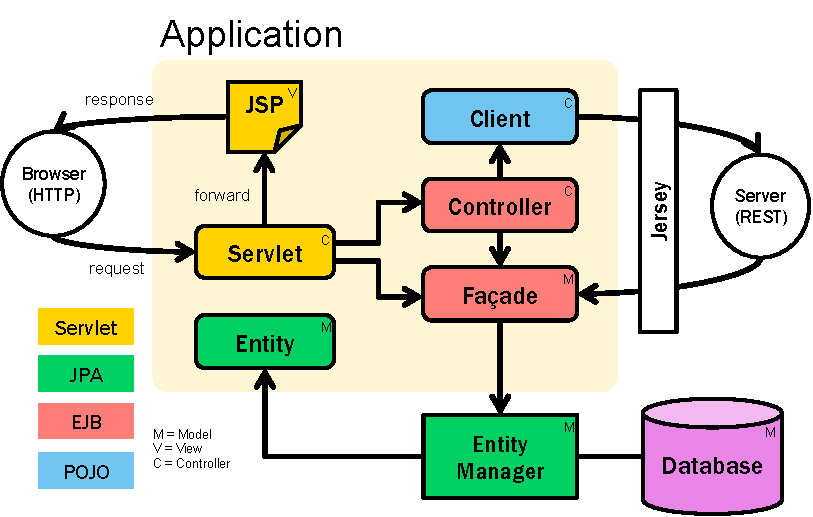
\includegraphics[scale=1]{img/architecture.pdf}  
\footnote{\textbf{JSP} JavaServer Pages}
\footnote{\textbf{JPA} Java Persistence API}
\footnote{\textbf{EJB} Enterprise Java Bean}
\footnote{\textbf{POJO} "Plain Old Java Object"}
\end{center}

The blocks represent modules in the system, and the thick lines show dependencies in the system.\\
The different colours of the modules indicate what kind of class they are.
Here is a brief overview of the concept:
\begin{itemize}
\item Data objects are defined as \textbf{Entity} classes. Entity objects are persisted to and retrieved from a database by the Java Persistence API.
\item The application retrieves and persists Entity objects via \textbf{Facade} classes.
\item Application logic is implemented in \textbf{Controllers}
\item User's browsers will invoke \textbf{Servlets} when they request a web page. Servlets respond to requests for data and actions. They request simple data transactions through Facades, and can defer more logical operations through Controllers.
\item The servlet's response gets forwarded to a related \textbf{JSP} page, which describes the view (the web page). When the JSP gets run, the data forwarded to it by the Servlet is inserted into the page in place of JSP tags.
\item Where data is required from multiple types of entities, facades can talk to other facades, and controllers can to other controllers where appropriate.
\item Other compatible servers can request data via a REST protocol, which special Service Facades handle. When this server wants to request data from another server, it does so through a Client class.
\end{itemize}

\clearpage
\subsection{Design Patterns}

\paragraph{Model-View-Controller}
Web applications by their very nature lean towards an MVC design paradigm. The view is the user's web browser, the controller is the application code and the model is the database. Not only this but MVC is a very robust and well proven pattern for designing applications. So MVC will be used throughout the design of the application.\\

To ensure MVC is correctly used, it should be very clear what packages, classes and other content does and doesn't do. The aim is to keep the Model, View and Controller implementation separate, so that, for example, model classes don't dictate how the data should look in a web page, that is the job of the view.

\paragraph{Facades}
The facade pattern will also be used as an extension of the Model to provide clean interfaces to the data. Facades will abstract away the details of persisting, retrieving and managing data from the database. By doing this, it prevents code related to database access from being spread across the application where access to data is required. Entity objects can be searched for, retrieved and persisted through single methods, rather than having JPA boilerplate code wherever entities need to be accessed.\\

Another advantage to using facades is that you can have multiple facades for the same set of data for different purposes. There will be facades for accessing data from within the application, and facades for accessing data over the inter-server REST protocol.

\paragraph{REST}
Representational State Transfer (ReST) will be used for inter-server communication with other group's servers. By using a set standard of API's, ReST allows easy access to data through standard HTTP methods. A client (whether it be a web browser or another application) can access data through URIs. By using standard HTTP methods, such as GET, POST and DELETE, this data can be accessed and manipulated without any special proprietary interfaces. The application will implement REST APIs through facades, where methods are invoked when a URI is requested, in a similar way that Servlets are instantiated when URLs are requested. Through the facade, data is returned, or processed depending on the method invoked. Entities will be serialised to JSON (Java Serialised Object Notation) object strings before being sent over REST. The application expects JSON object strings from other servers also, and they must be de-serialised back into entity objects.

\paragraph{EJB}
Controller and Facade classes are Enterprise Java Session Beans. This basically means that instances of those classes are handled by the Java EE runtime in Glassfish. Session Beans are not instantiated when they are needed, instead instances that are shared among multiple sessions are 'injected' into the dependant class. This reduces system resources, as there could be many sessions at once, instantiating the same class. Instead there is one instance for the application, shared among sessions.

\subsection{Required libraries}
The application should not require any libraries which are not available as part of a standard Java EE stack. The development environment, NetBeans, provides a full Java EE stack to develop from, including common libraries which may not be part of the Java EE distribution. There is one library which, while available with the standard NetBeans Java EE environment, needs to be explicitly included in the project. Other IDE's or distributions may not include this library, so it would need to be manually obtained and included in the build classpath.
\paragraph{Jersey 1.8}
Jersey is an open-source, production quality library for building RESTful web services in Java. It automatically handles the carriage of data over ReST to and from a Java EE application, and includes annotations which allow the invocation of methods when ReST resources are requested. It also includes \textbf{Jackson}, the most popular and probably best JSON serialiser/parser, and it automatically works with the ReST services provided in Jersey.\\

Jersey 1.8 is available in the latest version of NetBeans as an optional library with can be included in the project.\\

It can also be obtained from \textbf{jersey.java.net}

\clearpage
\section{Packages and significant classes}
Classes in the application are organised in packages, where each class of a certain type are in the same package. Classes in packages are expected to depend on and interact with other classes in other packages, so packages are not used for scope, just organisation.\\

This section describes each package and what the classes in those packages are expected to do. It also describes each class in the package, and gives a interface description of significant classes.

\subsection{Entity package}
Entity classes define a data object which can be persisted to a database via JPA. Refer to \textbf{Section 4 Data Entity Design} for a description of these classes and how they should be used.

\subsection{Servlet package}
Servlet classes are invoked when a client requests a "page" in the application. The servlet mapped to the URL address gets instantiated and is tasked with responding to a HTTP request. The request may contain posted data, such as that from a form. It is the servlet's job to call methods in other parts of the application to respond appropriately to a request, and to get the data that will be required in the response. The design of the servlets in this application is not to produce the 'view' of the response, instead it forwards the data it has obtained to a JSP page. In this sense a servlet a view controller.\\

All servlets extend the Java EE class \texttt{HttpServlet}, which defines the methods which get invoked for each HTTP method that a client can access, such as \texttt{GET} and \texttt{POST}. A servlet should override the appropriate methods to provide the service that the servlet is expected to provide. They can have any other methods as well, but should defer significant application logic to the appropriate Controller classes where appropriate.
A servlet should not output any HTML in its response to a \texttt{GET} request. Instead, all HTML should defined in a JSP page for a particular servlet.\\

To produce a visible page to a user's web browser, a servlet should override the \texttt{doGet} method. It should obtain any data that it needs to display to the user through Controllers and/or Facades, store the retrieved data in 'attributes' of the passed in \texttt{HttpServletRequest} object, then forward that request to the appropriate JSP page, where the JSP reads the attributes and inserts the data into it's HTML content, which arrives at the user's browser.\\

Here is a simple example of a servlet in the prototype, \texttt{ServersServlet}:
\begin{small}\begin{verbatim}
@WebServlet(name = "Servers", urlPatterns = {"/Servers"})
public class ServersServlet extends HttpServlet {

    @EJB
    ServerFacade serverFacade;

    @Override
    protected void doGet(HttpServletRequest request, HttpServletResponse response) {
    	List<Server> servers = serverFacade.findAll();
    	request.setAttribute("servers", servers);
    	request.getRequestDispatcher("servers.jsp").forward(request, response);
    }

    @Override
    protected void doPost(HttpServletRequest request, HttpServletResponse response) {
    	String name = request.getParameter("name");
    	String serviceRootURL = request.getParameter("serviceRootURL");
    	
    	Server server = new Server(name, serviceRootURL);
    	serverFacade.create(server);
    	
    	doGet(request, response);
    }
}
\end{verbatim}\end{small}


There will be a servlet for each 'page' in the application, so for example the login page will have a LoginServlet.
All servlets will be similar to the example above, retrieving entity data through a facade to forward to a JSP, and responding to \texttt{POST} requests by creating entities, persisting them through a facade, or invoking methods in a Controller, using parameters in the request object.

\subsection{Controller package}
Controller classes contain the majority of the application's logic. They define it's behaviour. While simple tasks can be performed in a servlet class, more complex behaviour and functionality which may need to be used in multiple servlets should be contained in a controller class. The object-oriented design of the application is such that there should be individual controllers for each type of entity being used and manipulated. In other words, there should be a Controller class for each Entity class, should it require one.\\

There are also special controllers which control other aspects of the application, like handling user login.\\
All controller classes should have \texttt{@Stateless} annotations to make them Stateless Session Beans, which can be injected into dependent classes using the \texttt{@EJB} annotation. They should not have to be instantiated each time they need to be used.



%\paragraph{UserController} Controls user operations. A lot of user operations, such as creation, updating and verification can be done through the facade, as these are standard data operations, but there are a few special operations that make more sense in a controller, such as managing a user's money.
\paragraph{FriendshipController} Controls friendship operations, like creating friend requests, accepting/rejecting friend requests and deleting friend requests. This controller will also invoke the FriendshipClient class, to send friendship information to remote servers via REST.

\begin{small}\begin{verbatim}
@Stateless
public class FriendshipController {
    @EJB FriendshipFacade friendshipFacade;
    @EJB ServerFacade serverFacade;
    
    public Friendship createFriendRequest(User localUser, String remoteUserId, Server remoteServer);
    public Friendship createFriendRequest(String localUserId, String remoteUserId, String remoteServerId);
    public boolean acceptRequest(Friendship f);
    public void unfriend(Friendship f);   
}
\end{verbatim}\end{small}

%Marcus
\paragraph{MonsterController} The MonsterController controls the different aspects that affect monsters, including the change of monster statistics over time, battles, breeding, genetics, and buying/selling monsters.
As a result, this class is also responsible for the creation of Monster objects: as this class contains the methods for randomisation, this will be used to randomise and vary the base attributes of the monster, as well as selecting a parent monster to inherit genes from if any.
\begin{small}\begin{verbatim}
@Stateless
public class MonsterController {
    public static Monster generate();
    public static Monster breed(Monster m1, Monster m2);
    public static Monster fight(Monster m1, Monster m2);
    public static double baseHealth(Monster m);
    public static double health(Monster m);
    public static double strength(Monster m);
    public static double dodge(Monster m);
}
\end{verbatim}\end{small}
%/Marcus
\paragraph{SessionController}
The SessionController controls user login, logoff and retrieval of information about the logged in user for a passed in HTTP session object.
\\A HTTP Session object is passed to a servlet as part of the request. It persists between requests as long as the user's web browser stays open. We store information about the logged in user in these sessions, specifically, a \textbf{User} entity object.
\\The methods in this class expect a \texttt{HttpSession} object, which can be retrieved from the \texttt{HttpServletRequest} object that gets passed in to a servlet method.
\begin{small}\begin{verbatim}
@Stateless
public class SessionController {
    @EJB UserFacade userFacade;
    
    public User getSessionUser(HttpSession session);
    public boolean verifySessionUser(HttpSession session);
    public boolean login(HttpSession session, String username, String password);
    public void logoff(HttpSession session);
}
\end{verbatim}\end{small}


\subsection{Facade package}
Facades are classes which expose and simplify the functionality for retrieving and persisting data entities to and from the database. It abstracts the JPA side of the application away from the rest of the app, reducing dependencies and providing a single interface to data so that data persistence code does not get spread across different parts of the architecture. Through a facade you can do core data transactions, such as retrieving, persisting, updating and removing Entity objects, but by having a facade for each entity, you can provide special convenience methods which make sense for that particular entity. For example, the friends facade can retrieve a list of friendships of a particular user, or the monsters facade can retrieve a list of monsters for a particular user.\\
There are two kinds of facade in the application, one to manage entities internally within the application, and one to provide access to data for the REST service. These two kinds of Facade are organised into their own sub-package of the Facade package: Session and Service.

\paragraph{AbstractFacade}
There is an abstract facade class which all Facade classes should extend. It provides common data access operations for any entity class, such as retrieving all objects in the database, persisting new objects, removing them etc.

\begin{small}\begin{verbatim}
public abstract class AbstractFacade<T> {
    private Class<T> entityClass;

    public AbstractFacade(Class<T> entityClass);

    protected abstract EntityManager getEntityManager();
    
    \* Persist a new entity object *\
    public void create(T entity);
    
    \* Persist an existing entity object *\
    public void edit(T entity);
    
    \* Remove a persisted entity object *\
    public void remove(T entity);
    
    \* Find a persisted entity object by unique database ID *\
    public T find(Object id);
    
    \* Find all persisted entities of this entity class *\
    public List<T> findAll();
    
    \* Find a range of persisted entities *\
    public List<T> findRange(int[] range);
    
    \* Count of all persisted entities *\
    public int count();
    
    \* Check that an entity object is 'valid' *\
    public boolean validate(T entity);
    
}

\end{verbatim}\end{small}
\textit{Note that \texttt{find(Object id)} does not find an entity by it's own identification attribute (like UserID), it finds it by it's automatically generated unique ID it inherits from AbstractEntity after being persisted to the database. See section 5}

\clearpage
\subsubsection{Session sub-package}
Session facade classes are facades for handling entity objects internally within the application. Each Entity class has a corresponding session facade class.

\paragraph{UserFacade}
Facade for the \textbf{User} entity. Validates user entities and has methods for retrieving user entities by user ID
\begin{small}\begin{verbatim}
@Stateless
public class UserFacade extends AbstractFacade<User> {
    @PersistenceContext(unitName = "MMP1PU")
    private EntityManager em;

    public boolean userIdExists(String userId);
    public User findByUserId(String userId);    
}
\end{verbatim}\end{small}

\paragraph{MonsterFacade}
Facade for the \textbf{Monster} entity. Validates monster entities and has methods for retrieving monster entities by monster ID.
\begin{small}\begin{verbatim}
@Stateless
public class MonsterFacade extends AbstractFacade<Monster> {
    @PersistenceContext(unitName = "MMP1PU")
    private EntityManager em;

    public List<Monster> findByUserId(String userId);
    public boolean monsterIdExists(String monsterId);
}
\end{verbatim}\end{small}

\paragraph{FriendshipFacade}
Facade for the \textbf{Friendship} entity. Validates Friendship entities and has many convenience methods for retrieving Friendships by various criteria.
\begin{small}\begin{verbatim}
@Stateless
public class FriendshipFacade extends AbstractFacade<Friendship> {
    @PersistenceContext(unitName = "MMP1PU")
    private EntityManager em;
    @EJB UserFacade userFacade;

	public Friendship find(String localUserId, String remoteUserId, String remoteServerId);
    public List<Friendship> findByLocalUserId(String localUserId);
    public List<Friendship> findReceivedRequests(String localUserId);
    public List<Friendship> findSentRequests(String localUserId);
    public List<Friendship> findFriends(String localUserId);    
}
\end{verbatim}\end{small}

\paragraph{ServerFacade}
Facade for the \textbf{Server} entity. Has one extra method to find a Server by it's name.
\begin{small}\begin{verbatim}
@Stateless
public class FriendshipFacade extends AbstractFacade<Friendship> {

    @PersistenceContext(unitName = "MMP1PU")
    private EntityManager em;
    
    public Server findByName(String name);
        
}
\end{verbatim}\end{small}

\subsubsection{Service sub-package}
Service facades are for producing and consuming data over the REST service. They have methods which respond to REST requests (like GET, PUT, POST) and produce and/or consume the data passed through the request and response of those methods.
\\Methods have special annotations from the Jersey REST library which describe how a method is invoked and how it should respond:
\\\texttt{\textbf{@GET @POST @PUT @DELETE}} Which HTTP method it will respond to
\\\texttt{\textbf{@Path("path/{arg}")}} Which path it will respond to and identified any parameters in that path
\\\texttt{\textbf{@Produces("application/json")}} The MIME type of the data that the method will produce (response)
\\\texttt{\textbf{@Consumes("application/json")}} The MIME type of the data that the method will consume (request)

\paragraph{UserFacadeREST} The REST service facade for users. Produces JSON representations of local users
\begin{small}\begin{verbatim}
@Stateless
@Path("users")
public class UserFacadeREST extends AbstractFacade<User> {

    @PersistenceContext(unitName = "MMP1PU")
    private EntityManager em;

    @GET
    @Path("{userId}")
    @Produces("application/json")
    public User findByUserId(@PathParam("userId") String userId);

    @GET
    @Produces("application/json")
    @Override
    public List<User> findAll();

}
\end{verbatim}\end{small}


\paragraph{FriendshipFacadeREST} The REST service facade for friendships. Responsible for receiving friend requests and request accepts and rejections from remote servers. Depends on \textbf{FriendshipFacade} (the session facade) for many Friendship entity lookup operations.
\begin{small}\begin{verbatim}
@Stateless
@Path("friend")
public class FriendshipFacadeREST extends AbstractFacade<Friendship> {

    @PersistenceContext(unitName = "MMP1PU")
    private EntityManager em;
    @EJB
    private UserFacade userFacade;
    @EJB
    private FriendshipFacade friendshipFacade;

    @POST
    @Consumes("application/json")
    public Response receiveFriendRequest(Friendship f);

    @POST
    @Path("{localKey}")
    @Consumes("text/plain")
    public Response setRemoteKey(@PathParam("localKey") String localKey, String remoteKey);

    @DELETE
    @Path("{key}")
    public Response remove(@PathParam("key") String key);

    @Override
    public boolean validate(Friendship f);
    
}
\end{verbatim}\end{small}

\clearpage
\subsection{Client package}
Client classes are for accessing REST resources on remote servers. They are for accessing information available through REST as well as posting information to other servers.

\paragraph{FriendshipClient} Sending, accepting and rejecting friend requests and deleting existing friendships.
\begin{small}\begin{verbatim}
public class FriendshipClient {

    public void sendFriendRequest(Friendship f);

    /* Post the local key of a friendship to it's remote server */
    public void sendKey(Friendship f);

    public void delete(String key);

}
\end{verbatim}\end{small}



\subsection{Filter package}
Filters are classes which, when the server is configured to do so, get invoked before every request for a servlet. They decide whether the request should continue or not, and can override the request by, for example, redirecting the user.
\paragraph{UserSessionFilter} This is the only servlet filter in the application, which ensures that most servlets can only be accessed when a valid user has logged in for the session. The application is configured on the server so that this filter is run during every servlet request. If a valid user exists in the HTTP session, it passes the request to the requested servlet, otherwise, it redirects the client to the Login servlet.\\
This class does not need to be used by any other part of the application, so an interface description is not included.

\subsection{Web folder}
Web content is not contained in a Java package like classes are, but will be part of the application in its own folder.\\
Web pages will be written as JSPs. JSP's are basically HTML files with special tags which contain instructions for the server to execute before it delivers the page to the client. The main use of these tags in the application will be to include data that has been forwarded to it from a servlet, and to iterate over that data, so that lists and tables can be dynamically generated. As well as these Java tags, everything that can be done in HTML files can be done in JSP's, such as CSS and JavaScript.

\subsection{Mapping from requirements to classes}

\begin{tabular}{|p{5cm}|p{11cm}|}
\hline 
\textbf{Requirement} & \textbf{Classes providing requirement} \\ 
\hline 
FR1 Server-based authentication & LoginServlet, RegisterServlet, UserSessionFilter, User, LocalUser, LocalUserFacade \\ \hline 
FR2 Server friends list & Friendship, User, FriendshipFacade, HomeServlet, FriendsServlet \\ \hline 
FR3 Server monster list & Monster, MonsterFacade, HomeServlet, MonstersServlet \\ \hline 
FR4 Server monster mash management & Monster, MonsterFacade, MonsterController \\ \hline
FR5 Server-server communication & Server, ServerFacadeREST, User, UserFacadeREST, Friendship, FriendshipFacadeREST, Monster, MonsterFacadeREST \\ \hline 
FR6 Client options & (Servlets) \\ \hline  
FR7 Startup of software in browser & LoginServlet, RegisterServlet \\ \hline  
FR8 Game display in browser & (Servlets), UserSessionFilter \\ \hline  
FR9 Friend matching & FriendsServlet, Friendship, FriendshipFacade, FriendshipFacadeREST, FriendshipClient, FriendshipController \\ \hline  
FR10 Fight notifications &  MonsterController, User, Monster\\ \hline  
FR11 Friends rich list &  User, UserFacade, FriendshipFacade\\ \hline  

\end{tabular} 


\clearpage
\section{Class Inheritance and Dependencies}
As described in the previous section, classes are organised into packages. The design of the packages group together classes of certain types. Classes in a package are expected to depend on and interact with classes in the same package and with classes in other packages.\\
It is virtually impossible to produce and include a UML class diagram of this application and have it fit on a piece of portrait A4. So the following UML diagram shows all of the classes and their packages, albeit without methods and attributes (Significant class methods are listed in Section 3), and shows the dependencies between facades and entities, and the dependencies of the FriendsServlet for example.

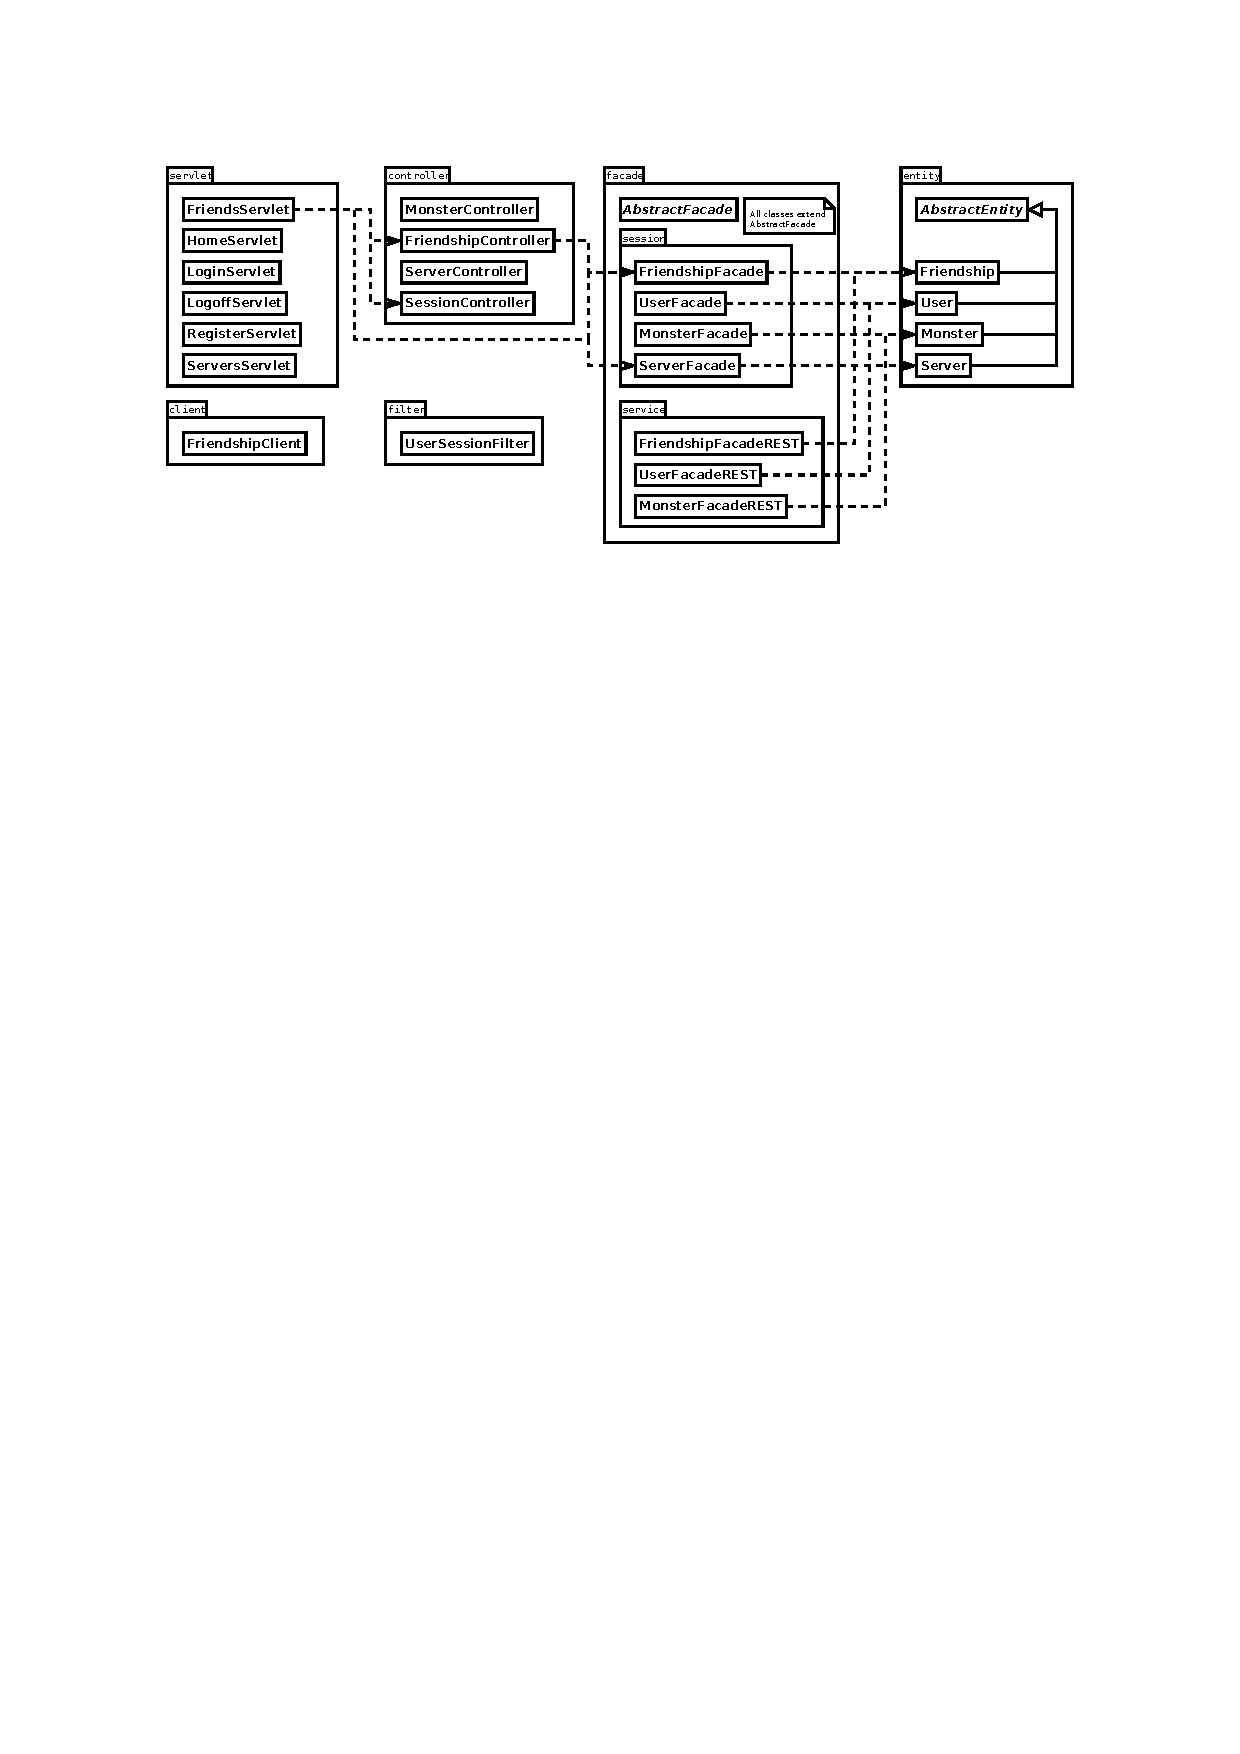
\includegraphics[scale=1.0]{img/dependencydiagram.pdf}

While we cannot deliver a complete UML diagram, we can describe a few design facts:
\\
\begin{itemize}
\item All entity classes have a corresponding session Facade class, so User will have UserFacade
\item The retrieval and persistence of Entity objects will be done via the Entity class' corresponding Facade class.
\item An Entity object, once it has been created, or obtained from a Facade, can be directly manipulated using it's accessors. The changes to that Entity object can then be persisted back to the database by passing it to the appropriate methods in the Entity's corresponding Facade.
\item There does not have to be a 'service' facade for each entity, only if the entities will be accessed via the ReST protocol
\item Controllers are stand-alone objects, in that they do not inherit from any other class
\item There will be a separate controller class for each entity, should one be required
\item Controller and Facade classes can depend on and interact with other controllers and facades, so that multiple types of entities can be used in the same place
\item Servlets can access and manipulate entity objects via corresponding controllers, facades, or a mixture of both
\item All Servlets extend the Java EE abstract class \textit{HttpServlet} and should override \textit{doGet} and if appropriate \textit{doPost}
\item Servlets should not depend on or interact with other servlet classes
\item Instances of Controller and Facade classes should be 'injected' into a depending class via EJB. In other words, a controller or a facade should not be instantiated when it is required by say a servlet for example. A single shared session instance of the classes should be obtained by using the \textbf{@EJB} annotation.
\end{itemize}

\clearpage
%\subsection{Servlet mapping and dependencies}
%This subsection lists every browsable page in the application, it's corresponding servlet, and which classes each servlet depends on.\\
%\begin{tabular}{|p{3cm}|p{3cm}|p{10cm}|}
%\hline
%\textbf{Web page}			& \textbf{Servlet}		& \textbf{Dependencies} \\
%\hline
%User's friends				& FriendsServlet		& FriendshipController, FriendshipFacade, ServerFacade \\
%\hline
%\end{tabular}



\clearpage
\section{Input/Output}

\textbf{*} Login \begin{math}\to\end{math} input: username, password \begin{math}\to\end{math} LoginServerlet.doGet(request, response) \begin{math}\to\end{math} output: sendRedirect or error\\

\textbf{*} Register \begin{math}\to\end{math} input: username, password, name \begin{math}\to\end{math} RegisterServerlet.doPost(request, response) \begin{math}\to\end{math} output: new User(username, name, password) or error\\

\textbf{*} Friends list \begin{math}\to\end{math} input: localUserId \begin{math}\to\end{math} FriendsFacade. findFriends(localUserId) \begin{math}\to\end{math} output: List\begin{math}<\end{math}Friendship\begin{math}>\end{math}\\

\textbf{*} Search friends \begin{math}\to\end{math} input: userId \begin{math}\to\end{math} UserFacade. findByUserId(userId) \begin{math}\to\end{math} output: User\\

\textbf{*} Requests (Friend invite) \begin{math}\to\end{math}  input: localUserId \begin{math}\to\end{math} FriendsFacade. findFriends(localUserId) \begin{math}\to\end{math} output: List\begin{math}<\end{math}Friendship\begin{math}>\end{math}\\

\textbf{*} Accept (Friendship) \begin{math}\to\end{math} input: localUserId, remoteUserId, remoteServerId, localKey, remoteKey \begin{math}\to\end{math} FriendshipController. acceptRequest(Friendship(localUserId, remoteUserId, remoteServerId, localKey, remoteKey)) \begin{math}\to\end{math} output: friend added\\

\textbf{*} Add friends \begin{math}\to\end{math} input: localUserId, remoteUserId, remoteServerId \begin{math}\to\end{math} FriendshipController. createFriendRequest(localUserId, remoteUserId, remoteServerId) \begin{math}\to\end{math} output: Friendship\\

\textbf{*} Remove friend \begin{math}\to\end{math} input: Friendship \begin{math}\to\end{math}  FriendshipController.unfriend(Friendship) \begin{math}\to\end{math} output: removed friend \\

\textbf{*} Monster List \begin{math}\to\end{math} ?? (input: localUserId \begin{math}\to\end{math} MonsterFacade.findMonsters(localUserId) \begin{math}\to\end{math} output: List\begin{math}<\end{math}Monster\begin{math}>\end{math})\\

\textbf{*} Requests (sell monster) \begin{math}\to\end{math} ?? (input: monsterId, price \begin{math}\to\end{math} MonsterController.sellMonster(monsterId, price) \begin{math}\to\end{math} output: )\\

\textbf{*} Requests (offer monster for breeding) \begin{math}\to\end{math} ?? (input: monsterId, price \begin{math}\to\end{math} MonsterController.offerBreeding(monsterId, price) \begin{math}\to\end{math} output: )\\

\textbf{*} Requests (monster breed) \begin{math}\to\end{math} input: maleMonsterId, femaleMonsterId) \begin{math}\to\end{math}  MonsterController.breed(maleMonsterId, femaleMonsterId) \begin{math}\to\end{math} output:  Monster\\

\textbf{*} Requests (loan monster) \begin{math}\to\end{math} ?? (input:  monsterId, price \begin{math}\to\end{math}  MonsterController.loanMonster(monsterId, price) \begin{math}\to\end{math} output: )\\

\textbf{*} Requests (monster battle) \begin{math}\to\end{math} ?? (input: localUserId, monsterId, remoteUserId, remoteMonsterId \begin{math}\to\end{math} MonsterController.requestBattle(localUserId, monsterId, remoteUserId, remoteMonsterId) \begin{math}\to\end{math} output: )\\

\textbf{*} Change monster name \begin{math}\to\end{math} ?? (input:  monsterName \begin{math}\to\end{math}  MonsterEntity.setName(monsterName) \begin{math}\to\end{math} output: changed name)\\

\textbf{*} Delete monster \begin{math}\to\end{math} ?? (input:  monsterId \begin{math}\to\end{math}  MonsterFacade.deleteMonster(monsterId) \begin{math}\to\end{math} output: deleted monster)\\

\textbf{*} Accept (buy monster) \begin{math}\to\end{math} ?? (input:  userId, monsterId \begin{math}\to\end{math} ??)\\

\textbf{*} Accept (monster battle) \begin{math}\to\end{math} input:  monster1, monster2 \begin{math}\to\end{math}  MonsterController.fight(monster1, monster2) \begin{math}\to\end{math} output: fight has occured\\ 

\textbf{*} Accept (breed monster) \begin{math}\to\end{math} ?? (input:  localUserId, monsterId, remoteUserId, remoteMonsterId \begin{math}\to\end{math}  MonsterController.breed(MonsterFacade.findMonsterById(monsterId), MonsterFacade.findMonsterById(remoteMonsterId)) \begin{math}\to\end{math} output:  Monster\\

\textbf{*} Accept (loan monster) \begin{math}\to\end{math} ?? (input:  userId, monsterId \begin{math}\to\end{math} ??)\\


\clearpage
\section{Data Entity Design}
Entity classes define a data object which can be persisted to a database via JPA. They have data fields and accessor methods only. They do not implement any logic, but have annotations which instruct the Java Persistence API and ReST API on how to handle individual fields of data.
\\
\begin{center}
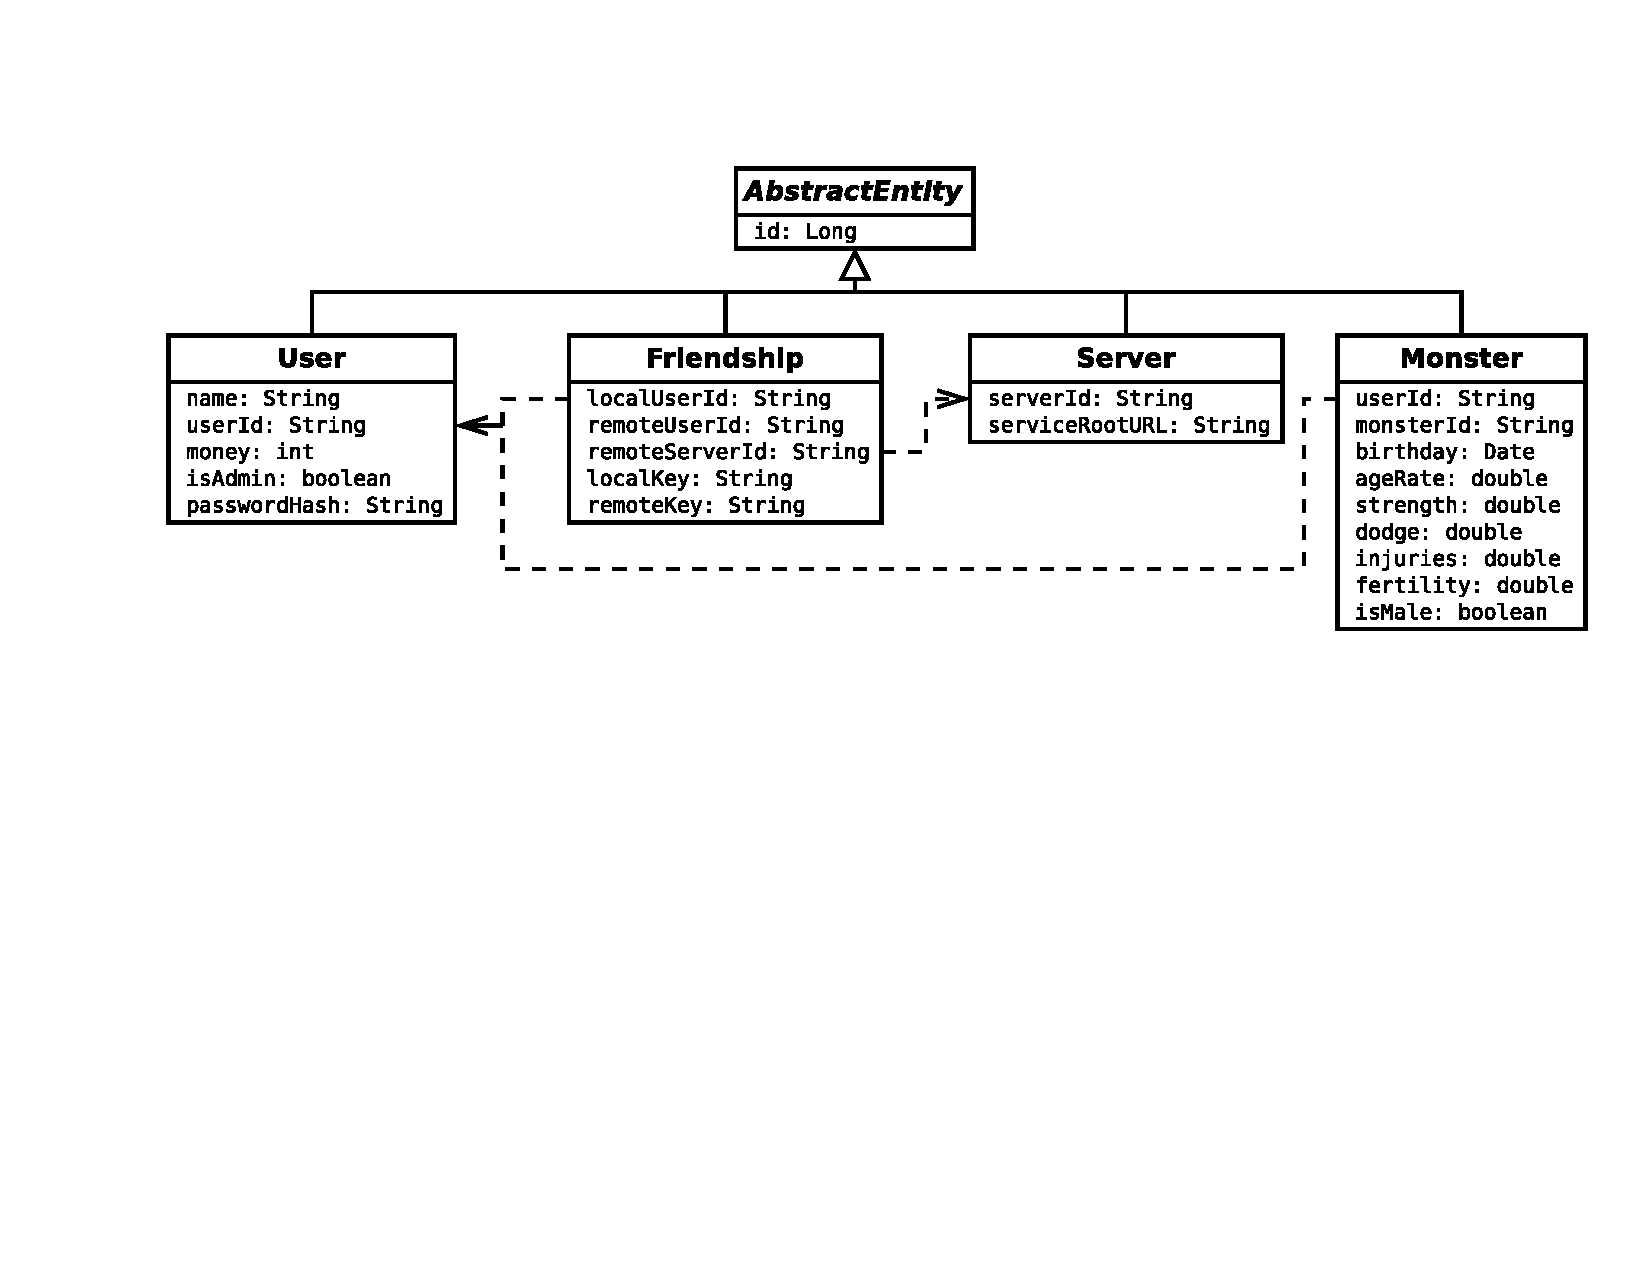
\includegraphics[width=\textwidth]{img/entitydiagram.pdf} 
\end{center}

This diagram describes the entity model design of the application. Each attribute which refers to another entity type is shown as a dashed line \textit{(see Relationships below)}.

\paragraph{Persistence}
Instances of entities (objects) are handled via the Entity Manager, which is provided by JPA and the Glassfish server. JPA talks to the database, and knows how to retrieve and persist these objects correctly. JPA automatically creates SQL tables based on the structure of an entity, eliminating the requirement for database design, as it can all be done by designing entities in Java. To simplify the process of retrieving and persisting Entity objects through JPA, Facade classes should be used instead of acquiring and interfacing with the Entity Manager directly, as described in Section 3.

\paragraph{Manipulation}
Entity objects can be created from scratch by simple instantiating an entity class, or an existing object can be retrieved from the database by using the entity's corresponding Facade.
\\Once you have an entity object instance, it's data can be directly manipulated through it's accessor methods.
\\The entity object can then be persisted to the database (as a new entity or updating the existing one) by passing it to the appropriate method in the Facade.

\paragraph{Relationships}
Relationships in the entity model are not hard coded in. That is, references to other types of entities are refereed to by an identifier attribute. For example, Friendship has a \textbf{localUserId} attribute, which should refer to a \textbf{User} entity via it's \textbf{userId} attribute.
\\The reason that entities do not have formal relationships (one-to-many, one-to-one etc) is that these entities need to be serialised and shared across ReST. By only having a referring ID as a reference to other entity types, this makes the entities more portable. Referenced entity objects can be obtained using lookup methods in the entity's correlating facade.

\paragraph{Annotations}
Entity classes make use of annotations, which describe how the data fields and accessors in the class should be used by JPA and the JSON serialiser for use in REST. JSON annotations are described in \textbf{AbstractEntity}.\\
One of the JPA annotations is \texttt{@NamedQuery}, which defines a JPQL (Java Persistence Query Language) query for this entity class. JPQL is similar to SQL. These are used by Facades to find and manipulate entities stored in the database. Multiple \texttt{@NamedQuery} annotations are contained in a \texttt{@NamedQueries} annotation. \\
Other JPA annotations specify whether fields are optional and whether their values should be unique in the database table, examples of which are in the interface descriptions below.

\clearpage
\subsection{AbstractEntity} An abstract entity which all entity classes should inherit and extend. AbstractEntity does not get persisted to the database, and has no use as a data object in the application.
\\The \textbf{id} attribute is an automatically generated, unique, long integer for uniquely identifying entity objects from the database. As each entity class inherits this attribute, it can be used to uniquely identity an entity object internally (e.g. in a JSP form), but is not much use beyond that.
\\The \texttt{@JsonAutoDetect(JsonMethod.NONE)} annotation instructs the JSON serialiser to ignore all properties by default. For properties to be serialised, they must be explicitly annotated to be so, or have the \texttt{@JsonAutoDetect} annotation overridden in a subclass, and instead choose properties to \textit{not} be serialised.
\begin{small}\begin{verbatim}
@MappedSuperclass
@JsonAutoDetect(JsonMethod.NONE)
public abstract class AbstractEntity implements Serializable {

    @Id
    @GeneratedValue(strategy = GenerationType.AUTO)
    @Basic(optional = false)
    private Long id;
    
    public Long getId();

}
\end{verbatim}\end{small}

\subsection{Server} References to remote servers. Contains their name, which should be unique across all compatible servers, and the URL from which REST services can be accessed.
\begin{small}\begin{verbatim}
@Entity
...
public class Server extends AbstractEntity {
    
    /* Fields */
    
    /* The unique identifier of the server.
     * This is what the server has decided to be named, and should be unique among all other servers.
     * Required */
    @Basic(optional = false)
    @Column(unique = true)
    private String name;
    
    /* The base URL of REST services of the server.
     * Requires a full URI description including the protocol.
     * For example "http://www.myserver.com:8080/myapp/webresources" */
    @Basic(optional = false)
    private String serviceRootURL;
    
    /* Constructors */
    
    public Server();
    public Server(String name, String serviceRootURL);
    
    /* Accessors */

    public String getName();
    public void setName(String name);
    public String getServiceRootURL();
    public void setServiceRootURL(String serviceRootURL);
}

\end{verbatim}\end{small}

\clearpage
\subsection{User}
Describes a user of the application or a compatible application with a different implementation. It has properties such as the user's name, their unique user ID, a hash of their password used to logon, and how much money the user has. This entity can be used to both represent 'local' users, that is users who have registered with and logon to this server, and remote users on other servers via REST, where not all attributes will have data (e.g. no password).
\\User entities which represent remote users should not be persisted to the database.
\begin{small}\begin{verbatim}
@Entity
...
public class User extends AbstractEntity {
    
    /* Fields */
    
    /* A unique identifier for the user. This should not change after the user is created.
     * Will be used by other entities to refer to this object.
     * Can be a short string like "jab41" or an email address for example. */
    @Basic(optional = false)
    private String name;
    
    /* The users real name. This is not a unique identifier. Not required.
     * Used as a more friendly representation of the user to others. */
    @Basic(optional = false)
    @Column(unique = true)
    private String userId;
    
    /* The amount of money the user has as an integer. Required to be at least 0. */
    @Basic(optional = false)
    private Integer money;
    
    /* A boolean indicating whether the user as administrative privileges,
     * and thus whether administrative facilities will be available to the user when logged on.
     * Required for local users only. Should default to false. Not exposed to REST. */
    @Basic(optional = false)
    private Boolean isAdmin;
    
    /* A SHA-1 hash of the user's password.
     * Plain-text passwords are never stored on the database, or used within the application.
     * Instead, passwords should be hashed by a one-way function (SHA-1).
     * To validate a password, hashes can simply be compared.
     * Required for local users only. Not exposed to REST. */
    private String password;
    
    /* Constructors */
    
    public User();
    public User(String userId, String name);
    public User(String userId, String name, String password);
    public User(String userId, String name, String password, boolean isAdmin);
    
    /* Accessors */
    
    @JsonProperty
    public String getName();
    public void setName(String name);
    @JsonProperty
    public String getUserID();
    public void setUserID(String userId);
    public Boolean getIsAdmin();
    public void setIsAdmin(Boolean isAdmin);
    public void setPassword(String password);
    public String getPasswordHash();
}
\end{verbatim}\end{small}

\clearpage
\subsection{Friendship}
Defines a 'friendship' between users. The entity references both a local user and another user, which can be local or remote. Users are referred to by the \textbf{UserID} attribute as defined in the \textbf{User} entity.
\\The server which the remote user is located on is specified by referring to a \textbf{Server} entity via the \textbf{remoteServerId} attribute.
\\Keys are used for handshake authentication between servers, so that friendships cant be manually 'forced'. The key exchange happens only when each user accepts the friend request, and those keys are used to validate operations that only friends can do.
\begin{small}\begin{verbatim}
@Entity
...
@JsonAutoDetect(JsonMethod.GETTER)
public class Friendship extends AbstractEntity {
    /* Fields */
    
    /* The userId of the local user of this friendship. Required. */
    @Basic(optional = false)
    private String localUserId;
    
    /* The userId of the user on the remote server. Required. */
    @Basic(optional = false)
    private String remoteUserId;
    
    /* The serverId of the server which hosts the remote user. Required. */
    @Basic(optional = false)
    private String remoteServerId;
    
    /* The key which the remote server requires to interact with the local user.
     * Not null only when the local user has accepted the friend request. */
    @Column(unique = true)
    private String localKey;
    
    /* The key which this server requires to interact with the remote user on the remote server.
     * Not null only when the remote user has accepted the friend request. */
    private String remoteKey;
    
    /* Constructors */
    
    public Friendship();
    public Friendship(String localUserId, String remoteUserId, String remoteServerId, String localKey,
                      String remoteKey);
    /* Methods */
    
    /* Is a local request (i.e. has been sent from a remote server) */
    public boolean isLocalRequest();
    
    /* Is a remote request (i.e. has been sent to a remote server) */
    public boolean isRemoteRequest();
    
    /* Is an accepted request (has both local and remote keys) */
    public boolean isAccepted();
    
    /* Accessors */

    public String getLocalUserId();
    public void setLocalUserId(String localUserId);
    public String getRemoteUserId();
    public void setRemoteUserId(String remoteUserId);
    public String getRemoteServerId();
    public void setRemoteServerId(String remoteServerId);
    public String getLocalKey();
    public void setLocalKey(String localKey);
    public String getRemoteKey();
    public void setRemoteKey(String remoteKey);   
}
\end{verbatim}\end{small}

\clearpage
\subsection{Monster} The Monster class acts as a hold for the Monster data. The data will be as static as possible, to prevent the need for multiple reads/writes from/to the database. The data stored in this class is: its time of birth (or birthday); its age rate (ageRate); its strength; its dodge-chance (dodge); any health deducted due to battle (injuries); its fertility; and finally, its gender.

\begin{small}\begin{verbatim}
@Entity
...
public class Monster extends AbstractEntity {
    
    /* Attributes */
    @Basic(optional=false)
    private String userId;
    
    @Basic(optional=false)
    @Temporal(TemporalType.DATE)
    private Date birthday;
    
    @Basic(optional=false)
    private double ageRate;
    
    @Basic(optional=false)
    private double strength;
    
    @Basic(optional=false)
    private double dodge;
    
    @Basic(optional=false)
    private double injuries;
    
    @Basic(optional=false)
    private double fertility;
    
    @Basic(optional=false)
    private boolean isMale;
    
    
    /* Constructors */
    public Monster();
    public Monster(double ar, double d, double s, double f, boolean m);
    
    /* Getters and setters */
    
    public String getUserID();
    public void setUserID(String id);
    public Date getBirthday();
    public void setBirthday(Date b);
    public double getAgeRate();
    public void setAgeRate(double ar);
    public double getStrength();
    public void setStrength(double s);
    public double getDodge();
    public void setDodge(double d);
    public double getInjuries();
    public void setInjuries(double i);
    public double getFertility();
    public void setFertility(double f);
    public boolean getIsMale();
    public void setIsMale(boolean m);
}
\end{verbatim}\end{small}


\clearpage
\section{Detailed Design}

\subsection{Significant algorithms}
\subsubsection{MonsterController}
\paragraph{Health and Life} Health determines how healthy a Monster is. It starts at 1 at birth and goes down to 0, at which point the monster dies. It will use the following formula:

Given \begin{math}d\end{math} is the date, \begin{math}b\end{math} is the monster's birthday, \begin{math}a\end{math} is the age rate, \begin{math}i\end{math} is the injury stat, \begin{math}B\end{math} is the base health and \begin{math}H\end{math} is the actual health:

\begin{math}
B = 2-exp((d-b)*a)\\
H = B-i
\end{math}

During battle, the amount of damage taken is decided from the other monster's strength stat, passed through a noise function that varies it.
\paragraph{Strength and Dodge} Strength is a stat that begins at 0 at birth, increases to max rate half-way through the age progression, then deteriorates again until reaching 0 at the end of the monster's natural life. The strength stat, combined with random noise, will determine how much damage will be dealt to the enemy monster per hit. It will use the following formula:

Given \begin{math}s\end{math} is the base strength and \begin{math}S\end{math} is the current strength:

\begin{math}
S = sB(exp(d-b)-1)
\end{math}

Dodge is a stat that, mathematically, is very similar to Strength. It determines the chances that a monster will dodge an attack. In order to determine whether the monster has dodged a given attack during battle, the dodge stat is combined with random noise and tested for whether it is above a given value. If it is, the dodge succeeds; if not, the damage is taken.
\paragraph{Breeding} Breeding will first test whether the monster will randomly mutate a stat and, if so, simply select a random value for the stat. If the monster will not randomly mutate the stat, it will select one of the two parents' stats to prefer, generate some noise for the stat and set that as the base of the stat for the new monster. The number of children generated will use the following formula:

given that \begin{math}n\end{math} is the number of children generated, \begin{math}M\end{math} is the maximum number of children any monster can have, \begin{math}f_{1}\end{math} is the fertility of the first parent and \begin{math}f_{2}\end{math} is the fertility of the second parent:

\begin{math}
n = M\sqrt{f_{1} * f_{2}}
\end{math}
\paragraph{Noise function} The noise function f will generate a random value between -1 and 1. It will be used in the following ways:
\begin{itemize}
\item{In a fight, the Strength attribute will be varied by \begin{math}S+(f*0.1)\end{math};}
\item{In a fight, the Dodge attribute will be varied by \begin{math}D+(f*0.5)\end{math};}
\item{In a fight, a successful Dodge will occur if the value returned by the above function is greater than 0.5;}
\item{During breeding, the preference of the parent for a given stat will be decided by whether the random number is positive or negative;}
\item{During breeding, a stat mutating randomly will be decided by whether the random number is less than -0.8;}
\item{During breeding, a mutating stat will be generated by \begin{math}\frac{f+1}{2}\end{math};}
\item{During the creation of a new random monster, the value of all stats will be decided by the above function.}
\end{itemize}


\clearpage
%--------------------------------------------------------------------

%\section{References}
%[1] \textit{Title of ref.} Author, version, etc.
%Reference here 
%\\ \relax \\ \relax

\section{Document History}
\begin{tabular}{| l | l | l | p{9cm} | p{2cm} |}
\hline
Version & CCF No. & Date & Changes made to Document & Changed by \\
\hline
0.1 & N/A & 22/11/12 & Initial draft & jab41\\
\hline
0.2 & N/A & 26/11/12 & Updated Application Architecture, added Data Entity Design, Inter-server Communication and Significant Algorithms:MonsterController & jab41, mah48\\
\hline
0.3 & N/A & 28/11/12 & Updated Decomposition Description, added Required libraries. Added Class Inheritance and Dependencies. Re-written Data Entity Design & jab41\\
\hline
0.4 & N/A & 01/12/12 & Restructuring. Included interface descriptions for all classes. Updated nearly every section. & jab41 \\
\hline
0.5 & N/A & 05/12/12 & Added Input/Output section. & kat15 \\
\hline
1.0 & N/A & 07/12/12 & Tidy up. & jab41 \\
\hline
1.1 & 1 & 07/12/12 & QA modifications - spelling/grammar. & sie5 \\
\hline
\end{tabular}
\end{document}